
\section{Objects and action in humans}

%%\subsubsection*{Objects and actions}

%\ifverbose
The example of the cross composed of prime numbers is a novel (albeit
unlikely) type of segmentation in our experience as adult humans.  We
might imagine that when we were very young, we had to initially form a
set of such criteria to solve the object identification/segmentation
problem in more mundane circumstances. 
%\else
%Humans are experts at solving the figure/ground problem, and
%segmenting objects out from their background.
%\fi
%
That such abilities
develop and are not completely innate is suggested by results in
neural science. For example Kovacs~\cite{kovacs00human} has shown that
perceptual grouping is slow to develop and continues to improve well
beyond early childhood (14 years). Long-range contour integration was
tested and this work elucidated how this ability develops to enable
extended spatial grouping.

\ifverbose
The pattern of interconnections in the visual cortex is also known
to complete development postnatally from cell staining methods
studies~\cite{burkhalter93development,callaway92development}.
Brown~\cite{brown94vision} argued that a developmental process, that
is one of structure formation, is involved in acquiring visual
abilities rather than a pure parameter adaptation procedure as in
machine learning algorithm.
\fi 

%Key to understanding how such capabilities could develop is the
A useful concept to understand how such capabilities could develop is the
well-known theory of Ungerleider and Mishkin~\cite{ungerleider82two}
who first formulated the hypothesis that objects are represented
differently during action than they are for a purely perceptual task.
Briefly, they argue that the brain's visual pathways split into two
main streams: the dorsal and the ventral~\cite{milner95visual}. The
dorsal deals with the information required for action, while the
ventral is important for more cognitive tasks such as maintaining an
object's identity and constancy.  Although the dorsal/ventral
segregation is emphasized by many commentators, it is significant that
there is a great deal of cross talk between the streams.  Observation
of agnosic patients~\cite{jeannerod97cognitive} shows a much more
complicated relationship than the simple dorsal/ventral dichotomy
would suggest.  For example, although some patients could not grasp
generic objects (e.g.  cylinders), they could correctly preshape the
hand to grasp known objects (e.g. a lipstick): interpreted in terms of
the two pathways, this implies that the ventral representation of the
object can supply the dorsal stream with size information.

%
%
\begin{figure}[tb]
\begin{center}
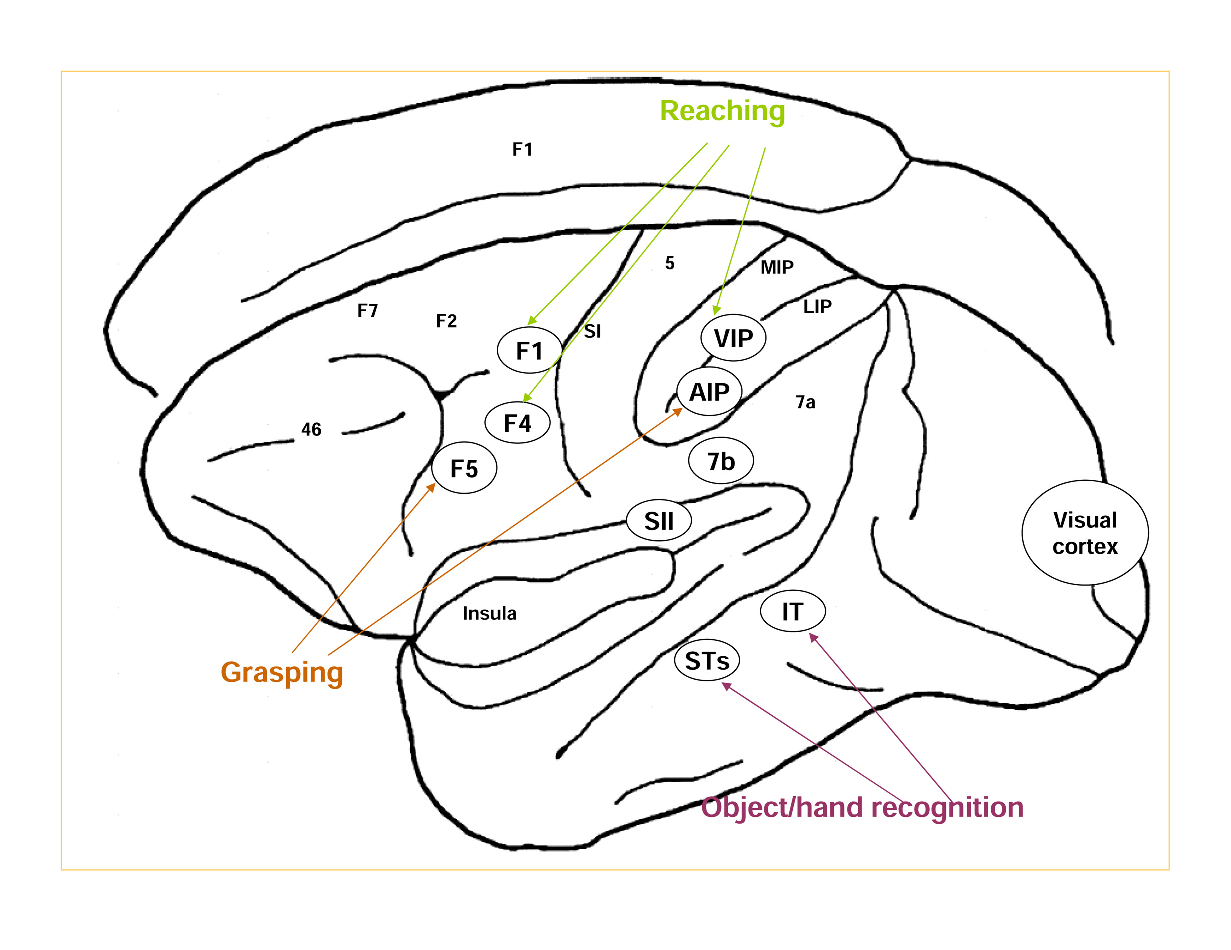
\includegraphics[width=10cm]{brain-schema.eps}
%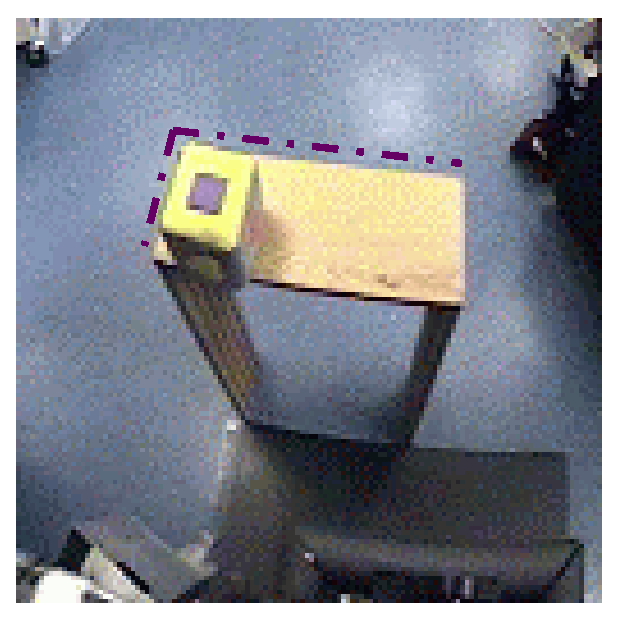
\includegraphics[width=\columnwidth]{setup-sequence.eps}
%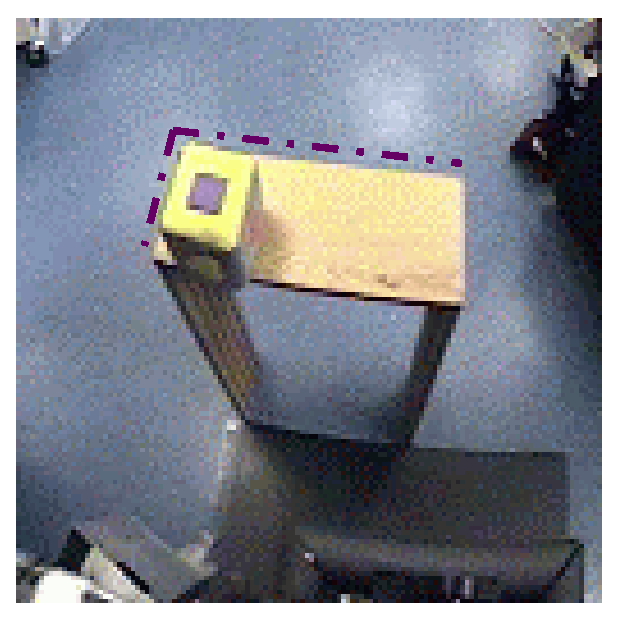
\psfig{file=setup-sequence.eps,width=4cm}
\caption{ 
\label{fig:brain-schema}
%
Monkey brain with indication of the main areas participating in object
oriented actions (adapted from~\cite{fagg-arbib-1998}). As described in the
text, three main functions can be identified: object recognition, reaching,
and grasping. These form three parallel yet connected streams of 
processing. The circuit connecting the visual cortex to the inferior parietal 
lobule (VIP/LIP), F4 and F1 subserves reaching (FIXIT unclear). AIP and F5 are responsible for
grasping. Temporal areas (TE, TEO) and STs are correlated to the
semantic of object recognition.
(FIXIT It's likely we need to ask permission to use this figure)
%
}
\end{center}
\end{figure}
%
%

Grossly simplifying, the brain circuitry responsible 
for object oriented actions is thought to consist of at least four 
interacting regions (Figure~\ref{fig:brain-schema}), namely the primary motor cortex (F1), the premotor cortex (F4, F5), the 
inferior parietal lobule (AIP, LIP), and the temporal cortex 
(TE, TEO)~(see \cite{rizzolatti-fogassi-gallese-1997,fadiga00visuomotor,jeannerod97cognitive} 
for a review). 
While this is a useful subdivision, it is worth bearing in mind 
that the connectivity of the brain is much more complex, that bidirectional 
connections are present, and that behavior is the result of a 
population activity of these areas. The example about the grasping of known 
objects in agnosic patients testifies to the \emph{abundance of anatomical connections} 
between different regions \cite{jeannerod-arbib-rizzolatti-sakata-1995}.

Another way of looking at the same connectivity is in terms of the main 
function of each area. For example F4, LIP, VIP, and 7b are involved in the control of 
reaching, F5 and AIP contain the majority of grasp related neurons, 
while TE and TEO are thought to subserve object recognition. These regions together form a network 
of parallel and yet interacting processes. In fact, at the behavioral level, it has 
been observed that reaching and 
grasping need to interact to correctly orient and preshape the hand~\cite{jeannerod-arbib-rizzolatti-sakata-1995}.

Neurons responsive to reaching are present in the inferior parietal lobule. For 
example, Jeannerod et al. reported 
that the temporary deactivation (FIXIT SUPPRESSION?) of the caudal part (VIP) of the intraparietal sulcus by injecting a GABA 
agonist
disrupts reaching~\cite{jeannerod-arbib-rizzolatti-sakata-1995}. Conversely, injection in the more rostral part (area AIP) 
interferes with the
preshaping of the hand. 

Some of the VIP neurons have bimodal visual and somatic receptive 
fields (RF). About 30\% of them have a RF which does not vary with 
movement of the head~\cite{rizzolatti-fogassi-gallese-1997}. The tactile and 
visual RF often overlap (e.g. a central visual 
RF corresponds to a tactile RF in the nose or mouth). The parietal cortex also contains 
cells related to eye position/movements that appear to be involved in  
the visuo-motor transformation required for reaching. VIP projects to area 
F4 in the premotor cortex. Area F4 contains neurons that respond to objects and 
are related to the description of the peripersonal space with respect to reaching~\cite{graziano-hu-gross-1997,fogassi96coding}. A subset of the F4 neurons 
have a somatosensory, visual, and motor receptive field. The visual receptive 
field extends in 3D from a given body part, such as the forearm. The somatosensory RF
is usually in register with the visual one (as in VIP neurons). Motor information
is integrated into the representation by maintaining the receptive
field anchored to the correspondent body part (the forearm in this
example) irrespective of the relative position of the head and arm.

Also, Graziano et al.~\cite{graziano-cooke-taylor-2000} described neurons that maintain a 
memory of the position of objects for the purpose of reaching. They found neurons 
that change their firing rate after an object is illuminated briefly
within reaching distance. The neurons return 
to their baseline firing rate only after the monkey is shown that the object have been 
taken away or moved to a different position.

Sakata and coworkers~\cite{sakata-taira-kusunoki-murata-tanaka-1997} 
investigated the response of neurons in the 
parietal cortex and in particular in area AIP (anterior intra-parietal). They found 
cells responsive to complex visual stimuli. Neurons in AIP responded during 
grasping/manipulative actions and when an object was presented to the 
monkey but no reaching was allowed. Neurons were classified as motor dominant, 
visual dominant or visuo-motor type depending on how they fired in the dark. Of 
the visual dominant neurons, some responded to the presentation of the 
object alone and often they were very specific to the size and orientation of the 
object, others to the type of object, while yet others responded indifferently to the 
presentation of a broad class of objects. Area AIP is interesting because 
it contains both motor and visually responsive cells intermixed in various proportions; 
it can be thought of as a visuo-motor vocabulary for controlling object directed 
actions. It is also interesting because projections from AIP terminate in the 
agranular frontal cortex. For many years, because of the paucity of data, this 
part of the cortex was considered just another area related solely to motor control. Recent studies 
(see~\cite{jeannerod97cognitive,fadiga00visuomotor}) have demonstrated 
that this is not the case. Particularly surprising was the discovery of visual 
responsive neurons. A good proportion of them have both visual/sensory and motor 
responses. Area F5, one of the main targets of the projection from AIP (to which 
it sends back recurrent connections), was thoroughly investigated by Rizzolatti 
and colleagues~\cite{gallese-fadiga-fogassi-rizzolatti-1996}.

%
%
\ifverbose
The dorsal stream goes through the parietal lobe and premotor cortex,
which project heavily onto the primary motor cortex to eventually
control movements. For many years the premotor cortex was considered
just another big motor area.  Recent studies~\cite{jeannerod97cognitive} have demonstrated that this is not the
case.  Visually responsive neurons have been found: some are purely
visual, but many have significant visuo-motor characteristics. In area
F5 in the monkey, neurons responding to object manipulation gestures
are found.  
\fi

F5 neurons can be classified in at least two different categories:
canonical and mirror (see Figure~\ref{fig:canonical-mirror}). 
Canonical and mirror neurons are 
indistinguishable from each other on the basis of their motor responses; 
their visual responses however are quite different. 
The canonical type is active in two situations:
i) when grasping an object and ii) when fixating that same object.
For example, a neuron active when grasping a ring also fires when the
monkey simply looks at the ring.  This could be thought of as a neural
analogue of the ``affordances'' of Gibson~\cite{gibson77theory}. 
However, given the heavy projection from AIP, it is not entirely
true that the affordances are fully described/computed by F5 alone.
A more conservative stance is that the system of AIP, F5, and other areas 
(such as TE) participate in the visual processing and motor matching required 
to compute the affordances of a given object.  


\begin{figure}[tbh]
\begin{center}
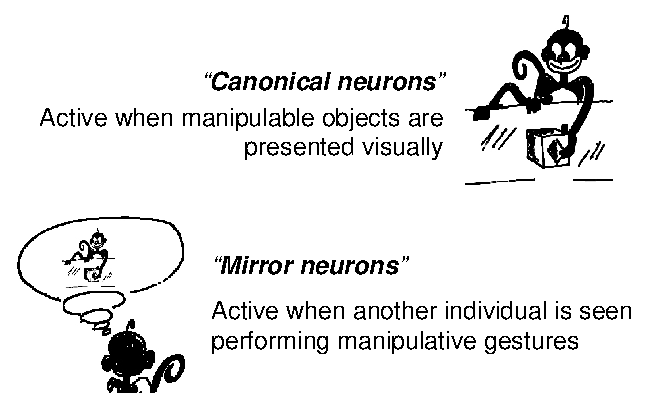
\includegraphics[width=10cm]{fig-canonical-mirror.eps}
\caption{ 
\label{fig:canonical-mirror}
%
Canonical and mirror neurons.
%
}
\end{center}
\end{figure}



\ifverbose
%
The affordances are a pragmatic action-related description of objects:
they can be seen as the properties of an object that can be exploited
by action.  For example a coffee mug has certainly a full palm
grasping affordance but also a precision grip one if using the handle
to lift it.
%
\fi

The second type of neuron identified in F5, the mirror neuron~\cite{fadiga00visuomotor}, becomes active under either of two conditions: i)
when manipulating an object (e.g. grasping it, as for canonical neurons), and ii) when watching
someone else performing the same action on the same object. This is a
more subtle representation of objects, which allows and supports, at
least in theory, mimicry behaviors. In humans, area F5 is thought to
correspond to Broca's area; there is an intriguing link between
gesture understanding, language, imitation, and mirror neurons~\cite{rizzolatti98language}.

The superior temporal sulcus region (STs) and parts of TE contain neurons
that are similar in response to mirror neurons~\cite{perret-mistlin-harries-chitty-1990}. 
They respond to the sight of the hand; the main difference compared to F5
is that they lack the motor response. It is likely that they participate in the 
processing of the visual information and then communicate with 
F5~\cite{gallese-fadiga-fogassi-rizzolatti-1996}.

A possible developmental explanation of the acquisition of
these functions can be framed in terms of tracing/interpreting chains 
of causally related events. Although it is still speculative, this analysis 
predicts that i) development of functions roughly follows a dorsal to ventral 
temporal gradient (i.e. reaching, grasping, recognition); ii) the 
ability to probe longer chains triggers the emergence of new functionality 
and/or a new set of behaviors. 
The next section delves deeper into
this proposal for the ontogenesis of object oriented action and
provides a hypothesis amenable to implementation.

\ifverbose
Also, looking at the three examples, we can notice 
a trend in complexity, and consequently we can hypothesize, that the time 
required to reach proficiency in each task is proportional to this complexity.
\fi

\ifverbose
Another important class of neurons in premotor cortex is found in area
F4~\cite{fogassi96coding}. While F5 is more concerned with the distal
muscles (i.e. the hand), F4 controls more proximal muscles (i.e.
reaching). A subset of neurons in F4 has a somatosensory, visual, and
motor receptive field. The visual receptive field (RF) extends in 3D
from a given body part, for example, the forearm. The somatosensory RF
is usually in register with the visual one. Finally, motor information
is integrated into the representation by maintaining the receptive
field anchored to the correspondent body part (the forearm in this
example) irrespective of the relative position of the head and arm.
\fi
